\chapter{Min-Weight Perfect Bipartite Matching} \label{chp:min_weight_perfect_bipartite_matching}

\section{Problem definition}
Given a weighted bipartite graph $G = (V, E)$ (remember that a bipartite graph is a graph whose vertices can be divided into two disjoint sets $V_1$ and $V_2$ such that every edge connects a vertex in $V_1$ to a vertex in $V_2$), let's define the concept of a matching.
\begin{definition}[Matching] \label{def:matching}
    A matching $M \in E$ is a collection of edges such that every vertex of $V$ is incident to at most one edge of $M$. In other words, a matching is a set of edges such that no two edges share a common vertex. 
\end{definition}

If a vertex $v$ has no edge of $M$ incident to it then $v$ is said to be exposed (or unmatched). A matching is perfect if no vertex is exposed; in other words, a matching is perfect if its cardinality is equal to $|V_1| = |V_2|$ \cite{goemans2009matching}.

\begin{figure}[H]
    \centering
    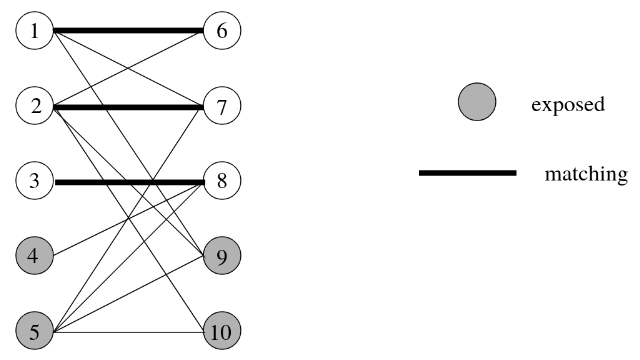
\includegraphics[width=0.6\textwidth]{Immagini/matching_example.png}
    \caption{Example of a perfect matching in a bipartite graph.}
    \label{fig:matching_example}
\end{figure}

The problem of finding a minimum weight perfect matching in a bipartite graph is a well-known problem in combinatorial optimization. The problem can be formulated as follows: 

\begin{definition}[Minimum weight perfect matching in bipartite graphs (\textsc{MWPBM})] \label{def:mwpbm}
    Given a weighted bipartite graph $G = (V, E)$, where $V = V_1 \cup V_2$ and $V_1 \cap V_2 = \emptyset$, find a perfect matching $M$ such that the sum of the weights of the edges in $M$ is minimized. The weight of a matching is the sum of the weights of the edges in the matching. The weight of an edge $e = (u, v)$ is denoted by $w(e)$. This problem is also called \textbf{the assignment problem}.
\end{definition}

\subsection{The existence of perfect matchings in bipartite graphs}
In this subsection a theorem is introduced that states a condition for the existence of perfect matchings in bipartite graphs. This theorem will be useful in the following chapter to proof our reduction \cite{viswanath2004perfect}.

Let's start with the definition of the \textbf{Tutte matrix} of a bipartite graph.
\begin{definition}[Tutte matrix] \label{def:tutte_matrix}
    The Tutte matrix of bipartite graph $G = (U, V, E)$ is an $n \times n$ matrix $M$ with the entry at row $i$ and column $j$
    \begin{equation}
        M_{i,j} =
        \begin{cases}
            0, & \text{if } (u_i, u_j) \notin E \\
            x_{i,j}, & \text{if } (u_i, u_j) \in E
        \end{cases}
    \end{equation}
\end{definition}

The determinant of the Tutte matrix is useful in testing whether a graph has a perfect matching or not, as the following theorem shows. 

\begin{theorem}[Existence of perfect matchings in bipartite graphs] \label {thm:perfect_matching_existence}
    Given a bipartite graph $G$ and the Tutte matrix $M$ for $G$ then the following equivalence holds:
    $$
    Det(M) \neq 0 \iff \text{There exists a perfect matching in G}
    $$
\end{theorem}

\begin{proof}
    We have the following expression for the determinant:

    $$
    \text{Det}(M) = \sum_{\pi \in S_n} (-1)^{sgn(\pi)} \prod_{i=1}^{n} M_{i,\pi(i)}
    $$

    where $S_n$ is the set of all permutations on $[n]$, and $sgn(\pi)$ is the sign of the permutation $\pi$. There is a one-to-one correspondence between a permutation $\pi \in S_n$ and a (possible) perfect matching 

    $$
    \{(u_1, v_{\pi(1)}), (u_2, v_{\pi(2)}), \cdots , (u_n, v_{\pi(n)})\} \text{ in } G.
    $$

    Note that if this perfect matching does not exist in $G$ (i.e., some edge $(u_i, v_{\pi(i)}) \notin E$), then the term corresponding to $\pi$ in the summation is $0$. So we have

    $$
    \text{Det}(M) = \sum_{\pi \in P} (-1)^{sgn(\pi)} \prod_{i=1}^{n} x_{i,\pi(i)}
    $$

    where $P$ is the set of perfect matchings in $G$. This is clearly zero if $P = \emptyset$, i.e., if $G$ has no perfect matching. If $G$ has a perfect matching, there is a $\pi \in P$ and the term corresponding to $\pi$ is

    $$
    \prod_{i=1}^{n} x_{i,\pi(i)} \neq 0.
    $$

    Additionally, there is no other term in the summation that contains the same set of variables. Therefore, this term is not cancelled by any other term. So in this case, $\text{Det}(M) \neq 0$.
\end{proof}

\subsection{Problem formulation}
The problem of finding a minimum weight perfect matching in a bipartite graph can be formulated as an integer linear program (ILP), i.e.an optimization problem in which the variables are restricted to integer values and the constraints and the objective function are linear as a function of these variables. Given a matching $M$, let $x$ be its incidence vector where $x_{ij} = 1$ if edge $(i, j)$ is in the matching, and $x_{ij} = 0$ otherwise. Then, the problem can be formulated as follows:

\begin{equation}
    \begin{aligned}
        \text{minimize} \quad & \sum_{(i, j) \in E} w_{ij} x_{ij} \\
        \text{subject to} \quad & \sum_{j \in V_2} x_{ij} = 1, \quad \forall i \in V_1 \\
        & \sum_{i \in V_1} x_{ij} = 1, \quad \forall j \in V_2 \\
        & x_{ij} \in \{0, 1\}, \quad \forall (i, j) \in E
    \end{aligned}
\end{equation}

Notice that any solution to this integer program corresponds to a matching and therefore this is a valid formulation of the minimum weight perfect matching problem in bipartite graphs.

The linear program relaxation of the above integer program is as follows:

\begin{equation}
    \begin{aligned}
        \text{minimize} \quad & \sum_{(i, j) \in E} w_{ij} x_{ij} \\
        \text{subject to} \quad & \sum_{j \in V_2} x_{ij} = 1, \quad \forall i \in V_1 \\
        & \sum_{i \in V_1} x_{ij} = 1, \quad \forall j \in V_2 \\
        & 0 \leq x_{ij} \leq 1, \quad \forall (i, j) \in E
    \end{aligned}
\end{equation}

The set of feasible solutions to the constraints in (P) forms a polytope. When optimizing a linear constraint over a polytope, the optimum will be achieved at one of the "corners" or extreme points of the polytope. An extreme point $x$ of a set $Q$ is an element $x \in Q$ that cannot be expressed as $\lambda y + (1 - \lambda) z$ with $0 < \lambda < 1$, $y, z \in Q$, and $y \neq z$. (This concept will be formalized and discussed in more detail when we cover polyhedral theory.)

In general, even if all the coefficients of the constraint matrix in a linear program are either 0 or 1, the extreme points of a linear program are not guaranteed to have all coordinates integral. This is not surprising since the general integer programming problem is NP-hard, while linear programming is solvable in polynomial time. Consequently, there is no guarantee that the value $Z_{IP}$ of an integer program is equal to the value $Z_{LP}$ of its LP relaxation. However, since the integer program is more constrained than the relaxation, we always have $Z_{IP} \geq Z_{LP}$, implying that $Z_{LP}$ is a lower bound on $Z_{IP}$ for a minimization problem. Moreover, if an optimal solution to a linear programming relaxation is integral, then it must also be an optimal solution to the integer program.

In our problem, the constraint matrix has a special form that lead to the following result: 

\begin{theorem}
    Any extreme point of ($P$) is a $0-1$ vector and, hence, is the incidence vector of a perfect matching.
\end{theorem}

Consequently, the polytope

\begin{equation}
    \begin{aligned}
        P = \{ x: & \sum_{j \in V_2} x_{ij} = 1, \quad \forall i \in V_1, \\
        & \sum_{i \in V_1} x_{ij} = 1, \quad \forall j \in V_2, \\
        & 0 \leq x_{ij} \leq 1, \quad \forall (i, j) \in E \}
    \end{aligned}
\end{equation}

is called the bipartite perfect matching polytope. 

\section{Solutions to the problem}
There are several algorithms to solve the problem of finding a minimum weight perfect matching in a bipartite graph. The first algorithm to solve this problem was proposed by Kuhn in 1955 \cite{kuhn1955hungarian}. The algorithm is based on the Hungarian method, which is a combinatorial optimization algorithm that solves the assignment problem in polynomial time. In the original paper the complexity of the algorithm was $O(n^4)$, but later Dinic and Kronrod \cite{dinic1969algorithm} showed that the algorithm can be implemented in $O(n^3)$ time.

The Hungarian method is a powerful algorithm, however, the algorithm is not very intuitive and can be difficult to implement. In recent years, several other algorithms have been proposed to solve the problem of finding a minimum weight perfect matching in a bipartite graph. In 1970, Edmonds and Karp \cite{edmonds1972theoretical} proposed an algorithm that solves the problem in $O(nm + n^2 \log n)$ time. In 1989 Gabow and Tarjan \cite{gabow1989faster} proposed an algorithm that solves the problem in $O(\sqrt{n}m \log(nW))$ time,  where $n,m$ and $W$ denote the number of vertices, number of edges, and largest magnitude of a cost; costs are assumed to be integral. The algorithms work by scaling. Lastly, in 2009, Sankowski and Piotr \cite{sankowski2009maximum} introduced a randomized algorithm that solves the problem in $O(Wn^w)$ time, where $w$ is the exponent of matrix multiplication, and $W$ is the highest edge weight in the graph.

In 2022, Chen, Li, et al. \cite{chen2022maximum} proposed a new solution to the Minimum-Cost Flow problem that woks in almost-linear time, precisely in $O(m^{1+o(1)})$ time. The minimum-cost flow problem is a classic combinatorial graph
problem that find numerous applications in engineering and
scientific computing. This result is important also for our problem, since the maximum weight perfect matching problem can be reduced to the minimum-cost flow problem, allowing to solve the problem in almost-linear time.

\section{Implementation used in this work}
In this section, we will present an implementation of the Gabow and Tarjan algorithm to solve the problem of finding a minimum weight perfect matching in a bipartite graph. The algorithm is based on scaling and is a generalization of the Hungarian method. The algorithm works by scaling the edge weights and then finding a perfect matching in the scaled graph. 
